\documentclass[../main.tex]{subfiles}
\graphicspath{{\subfix{../images/}}}
\begin{document}

  A etapa de resultados e análises tem como objetivo realizar testes e coletar dados para a análise de performance dos algoritmos implementados no robô. Durante essa etapa, será analisada a performance do robô no mundo real de forma estatistica, por meio de três testes. O primeiro consiste em observar a capacidade do protótipo em mover o pé por uma dada trajetória. No segundo teste é analisado se o robô atende a uma velocidade solicitada, utilizando dois terrenos diferentes e observando a oscilação de estabilidade do corpo ao longo da trajetória. Por fim, foi analisado a perfomance do Caramelo caminhando por terrenos inclinados e sua capacidade de ultrapassar pequenos obstáculos.

  \subsection{Cinemática Inversa}

  A partir das equações obtidas para a Cinemática Inversa do robô, o sistema é capaz não só de realizar a cinemática de cada uma das pernas individualmente, como também do seu corpo em todos os 6 graus de liberdade (translações em $x, y, z$ e rotações em $roll, pitch, yaw$). A figura \ref{fig:moving_body} ilustra o movimento do corpo do robô em cada um desses graus de liberdade.

  \begin{figure}[h]
    \centering
    \caption{Titulo da Figura}
    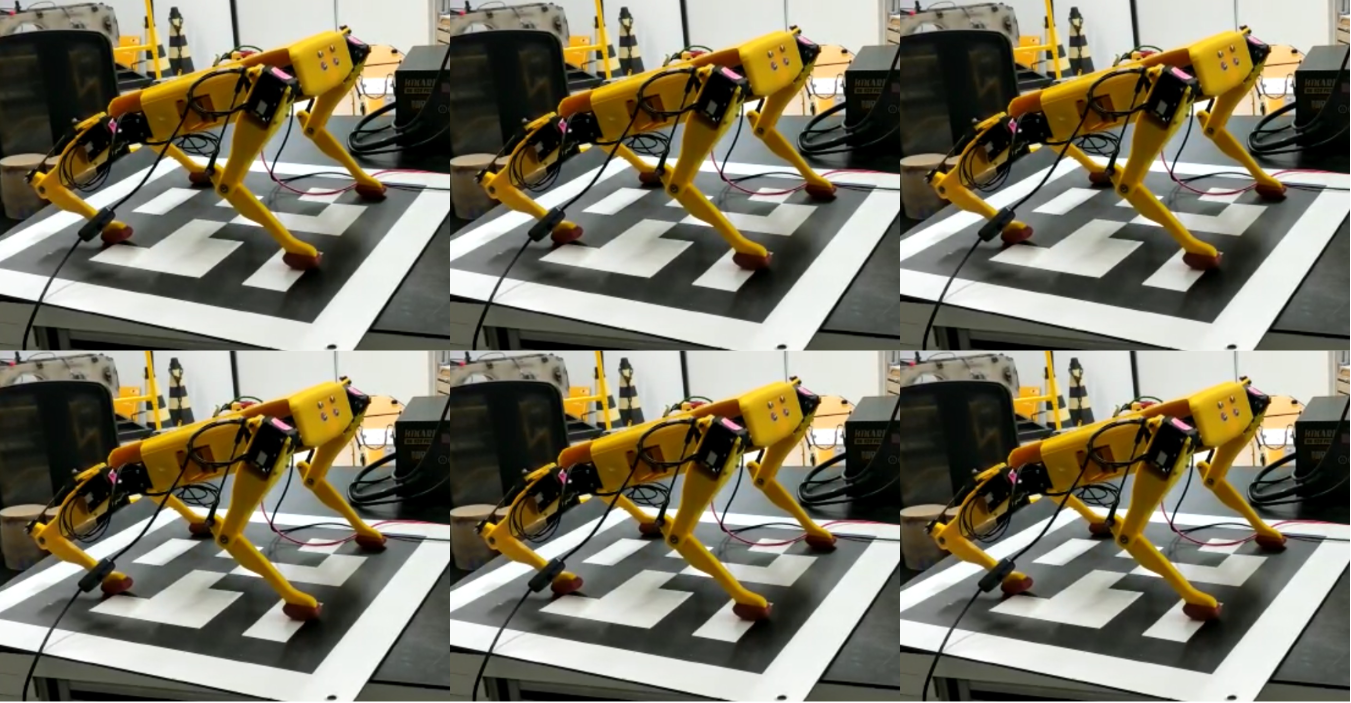
\includegraphics[width=0.48\textwidth]{moving_body.png}
    
    Fonte: XXX
    \label{fig:moving_body}
  \end{figure}

  \subsection{Controle de Rotação}

  Os gráficos da figura \ref{fig:grafico_controlling} ilustram o comportamento do sistema à variação dos \textit{setpoints} de orientação em $X$ (gráfico superior) e em $Y$ (gráfico inferior) para o corpo do robô, a partir da aplicação de diversos degraus (em azul). Nota-se que o protótipo é capaz de se adaptar rapidamente aos novos valores desejados de orientação, simultaneamente em ambos os eixos.

  \begin{figure}[h]
    \centering
    \caption{Titulo da Figura}
    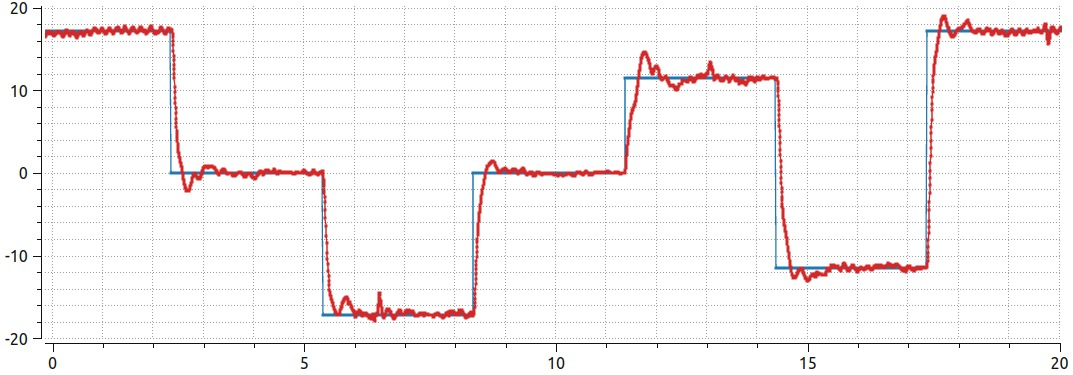
\includegraphics[width=0.48\textwidth]{grafico_controlling_X.png}
    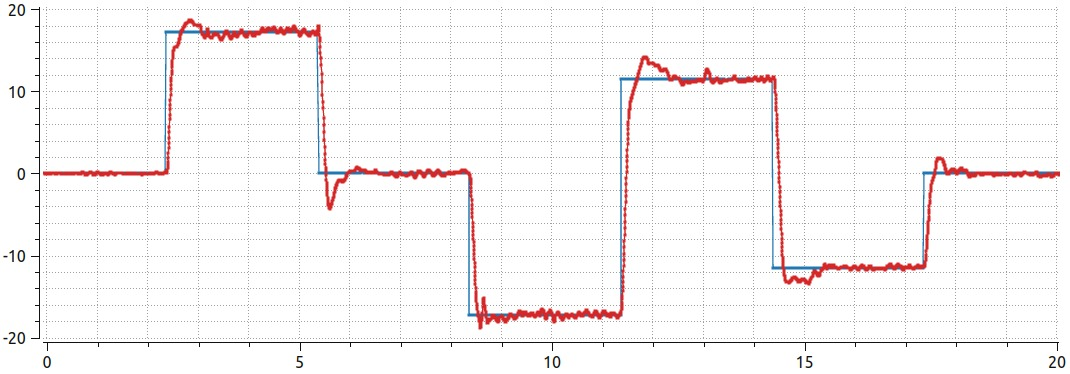
\includegraphics[width=0.48\textwidth]{grafico_controlling_Y.png}
    
    Fonte: XXX
    \label{fig:grafico_controlling}
  \end{figure}

  \subsection{Análise de trajetória}
  Durante este experimento, o corpo do protótipo está estático e suspenso por um suporte, sendo solicitado que uma de suas patas realize duas trajetórias calculadas pelo algoritimo proposto. Para geração das trajetórias foi considerado um período de $0.5 s$, altura do passo de $0.05 m$ e resolução de 25 pontos com distribuição homogênea, com deslocamentos em $(x, y)$ de $(0.05, 0.03)$ e $(0.03, 0.05)$ respectivamente, sendo realizados 30 testes para cada caso. 
  
  O objetivo aqui é analisar o tempo real de execução da trajetória, as coordenadas finais $(x_f, y_f)$ da pata e a altura máxima $z_{max}$ atingida durante o passo, comparando-os com os valores desejados para cada um desses parâmetros. A tabela \ref{tab:trajetoria} traz as médias encontradas para cada um desses parâmetros durante a realização dos testes.

  \begin{table}[h]
    \caption{Titulo da Tabela}
    \centering
      \begin{tabular}{lllll}
             & $tempo (s)$ & $x_{final}(m)$ & $y_{final}(m)$ & $z_{max}(m)$ \\
      Exp. 1 & 0.559457 & 0.050349 & 0.029247 & 0.047585 \\
      Exp. 2 & 0.556770 & 0.030240 & 0.049132 & 0.046562      
      \end{tabular}

    Fonte: Autoria própria
    \label{tab:trajetoria}
  \end{table}

  Inicialmente, foram realizados dois testes de T Student para amostras independentes, o primeiro relacionando o tempo de execução da trajetória nos experimentos 1 e 2, e o segundo relacionando a altura máxima alcançada, com o intuito de verificar se os resultados se alteram para diferentes valores $(x, y)$ desejados. O resultado da análise de T Student traz um $t$ de aproximadamente $1.087$, em se tratando de tempo, e de $1.0658$ para a altura máxima alcançada durante o passo. Para uma confiabilidade de $95\%$ e um total de 58 graus de liberdade, o valor crítico $t_c$ encontrado é de $2.00$. Como ambos os valores encontrados estão dentro do intervalo de confiança ($-t_c < t < t_c$), isso mostra que não há uma diferença significativa entre as médias em cada experimento, o que significa que diferentes comandos de trajetórias em $(x, y)$ não interferem nos resultados de tempo e altura máxima do passo.
  
  Os gráficos da figura \ref{fig:grafico_trajetoria_xyz} representam um dos testes realizados para o primeiro caso ($x=0.05m$, $y=0.03m$), sendo os gráficos superiores esquerdo e direito correspondentes à trajetória em $x$ e $y$ respectivamente, e o gráfico inferior correspondente à trajetória em $z$ (altura do passo). Nota-se que, como esperado pela análise da tabela \ref{tab:trajetoria}, há um atraso na execução da trajetória (neste caso específico de aproximadamente $54ms$) e a altura máxima alcançada é levemente inferior à desejada (alcançando neste caso um valor próximo a $0.0476m$).

  \begin{figure}[h]
    \centering
    \caption{Titulo da Figura}
    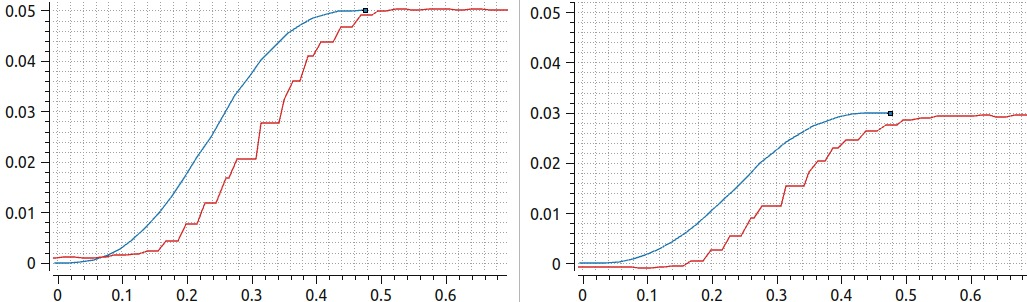
\includegraphics[width=0.48\textwidth]{grafico_trajetoria_xy.png}
    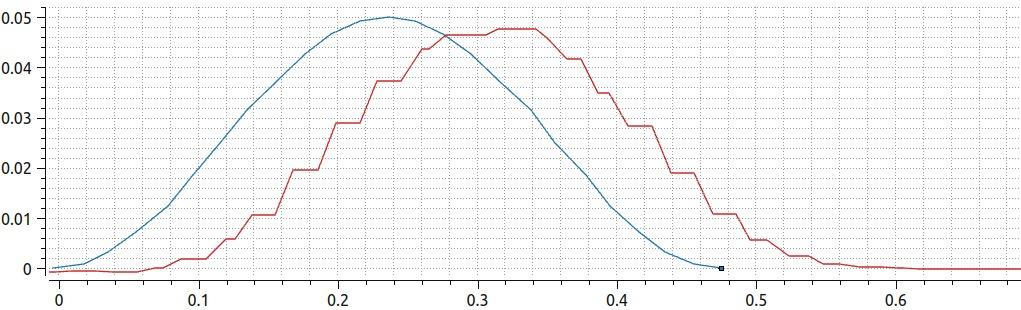
\includegraphics[width=0.48\textwidth]{grafico_trajetoria_z.png}
    
    Fonte: XXX
    \label{fig:grafico_trajetoria_xyz}
  \end{figure}

  \subsection{Controle de velocidade}

  Para o teste do controle de velocidade, foi enviado um comando de velocidade linear, na direção x, e medido o tempo que o robô levou para alcançar 1,5 m, dessa forma, obteve-se a velocidade média do robô. Neste experimento parte dos testes aconteceram utilizando o controle de estabilidade proposto e a outra parte sem, a fim de analisar a contribuição deste metódo no equilibrio do robô ao desempenhar uma trajetória. Os testes ocorreram com os mesmos paramêtros de passo do teste anterior, e em dois terrenos distintos, um terreno regular, feito de concreto e outro irregular, composto por pequenas pedras, como demonstra a imagem W.

  APRESENTAR TABELA E CONSIDERAÇÕES
  
  \subsection{Teste 3}
  Além dos testes realizados em terreno plano e irregular, o protótipo também foi submetido a 

\end{document}